\tikzset{
    position/.style args={#1:#2 from #3}{
        at=(#3.#1), anchor=#1+180, shift=(#1:#2)
    }
}

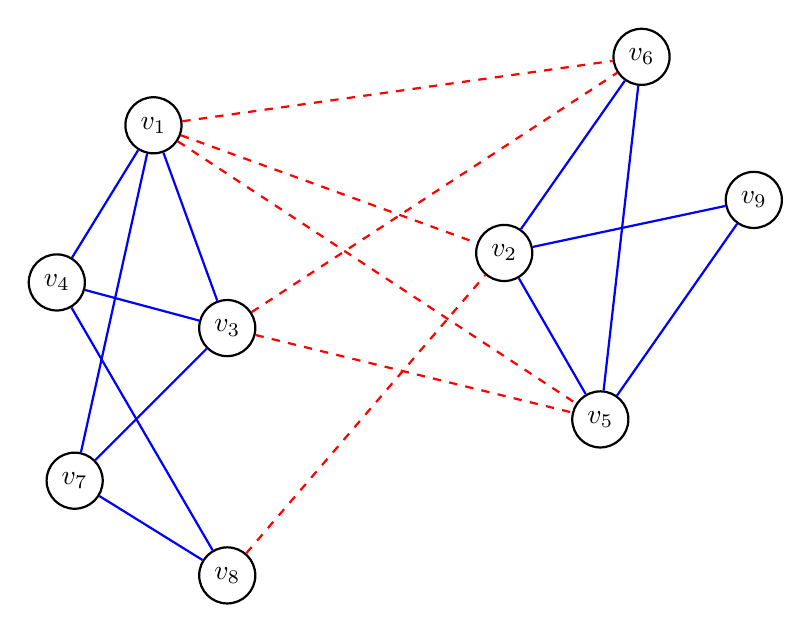
\begin{tikzpicture}

    \begin{scope}[every node/.style={circle,thick,draw}]
        \node (v1) at (0,0) {$v_1$};
        \node[position=-20:4cm from v1] (v2) {$v_2$};
        \node[position=-60:1.7cm from v2] (v5) {$v_5$};
        \node[position=55:2.3cm from v2] (v6) {$v_6$};
        \node[position=12:2.5cm from v2] (v9) {$v_9$};
        \node[position=-70:2cm from v1] (v3) {$v_3$};
        \node[position=-195:1.5cm from v3] (v4) {$v_4$};
        \node[position=225:2cm from v3] (v7) {$v_7$};
        \node[position=-90:2.4cm from v3] (v8) {$v_8$};
    \end{scope}

    % positive edges
    \begin{scope}[every edge/.style={thick,draw,blue},
        every node/.style={fill=white,circle}]
        % \draw (v4) -- (v1) -- (v3) -- (v2) -- (v1);
        \path 
        (v2) edge (v5) 
        (v5) edge (v9)
        (v2) edge (v6)
        (v6) edge (v5)
        (v2) edge (v9)      
        (v1) edge (v3)
        (v1) edge (v4)
        (v4) edge (v3)
        (v3) edge (v7)
        (v7) edge (v1)
        (v4) edge (v8)
        (v8) edge (v7)
        ;
    \end{scope}
    % negative edges
    \begin{scope}[every edge/.style={thick,draw,red,dashed},
        every node/.style={fill=white,circle}]
        % \draw (v4) -- (v1) -- (v3) -- (v2) -- (v1);
        \path 
        (v1) edge (v2)
        (v1) edge (v6)
        (v3) edge (v6)
        (v3) edge (v5)
        (v8) edge (v2)
        (v1) edge (v5)
        ;
    \end{scope}
  \end{tikzpicture}
  